\documentclass{article}
\usepackage[utf8]{inputenc}
\usepackage{titlesec}
\usepackage{amsmath}
\usepackage{listings}
\usepackage{subcaption}


\usepackage{graphicx}
\usepackage{placeins}
\graphicspath{ {images/} }

\title{Homework 4}
\author{Stephen Sullivan [sksulli2@illinois.edu]\\ Abhishek Modi [akmodi2@illinois.edu] }
\date{Spring 2016 \textbar\  CS 498 AML }

\begin{document}
\maketitle

\section{EM Topic Models}

\section{Image segmentation using EM}

\begin{figure}[ht!]
	\centering
	\caption{Nature 10}
	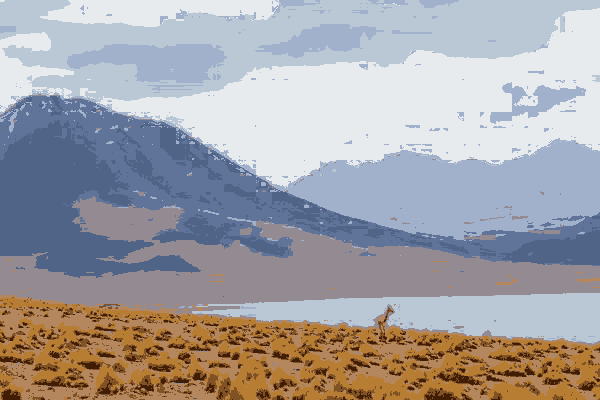
\includegraphics[width=90mm]{nature-em-k10-20.png}
\end{figure}

\begin{figure}[ht!]
	\centering
	\caption{Nature 20}
	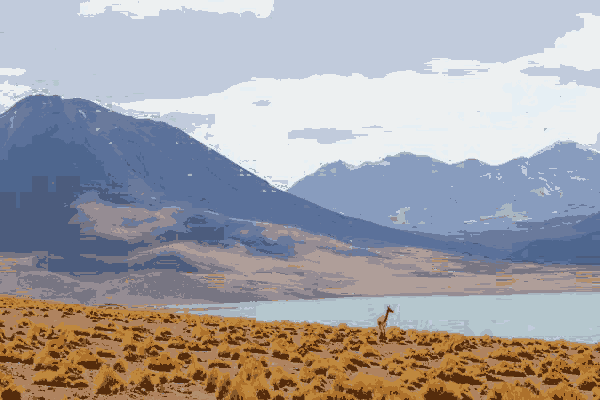
\includegraphics[width=90mm]{nature-em-k20-28.png}
\end{figure}

\begin{figure}[ht!]
	\centering
	\caption{Nature 50}
	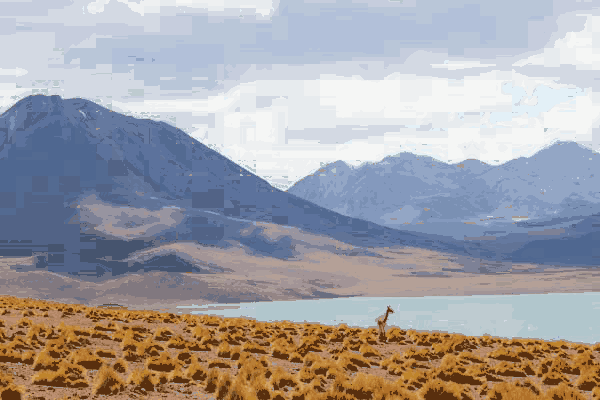
\includegraphics[width=90mm]{nature-em-k50-48.png}
\end{figure}

\begin{figure}[ht!]
	\centering
	\caption{Mountains 10}
	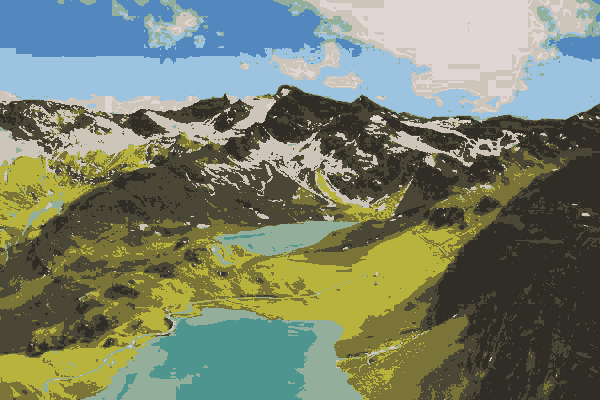
\includegraphics[width=90mm]{mountains-em-k10-24.png}
\end{figure}

\begin{figure}[ht!]
	\centering
	\caption{Mountains 20}
	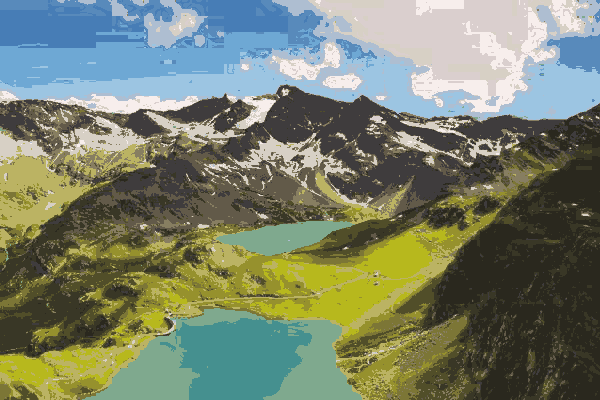
\includegraphics[width=90mm]{mountains-em-k20-44.png}
\end{figure}

\begin{figure}[ht!]
	\centering
	\caption{Mountains 50}
	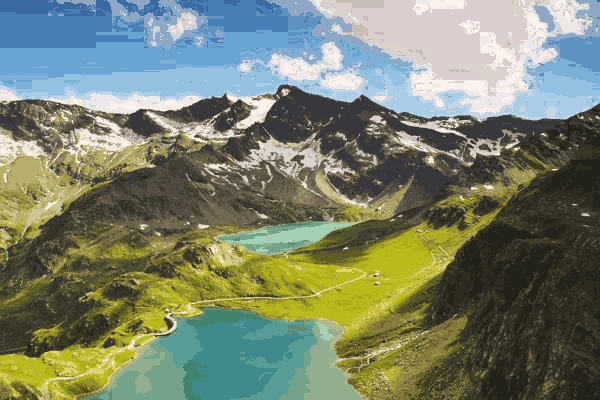
\includegraphics[width=90mm]{mountains-em-k50-21.png}
\end{figure}


\begin{figure}[ht!]
	\centering
	\caption{Ocean 10}
	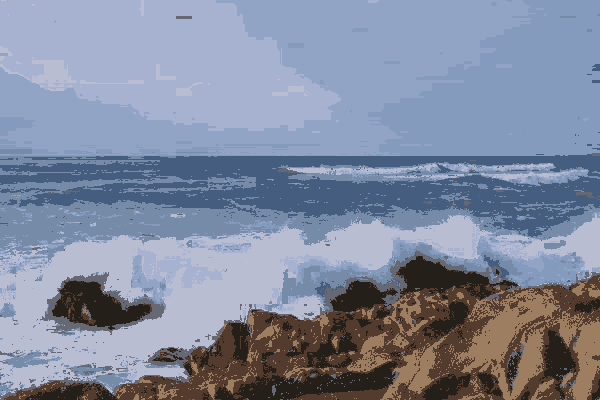
\includegraphics[width=90mm]{ocean-em-k10-29.png}
\end{figure}

\begin{figure}[ht!]
	\centering
	\caption{Ocean 20}
	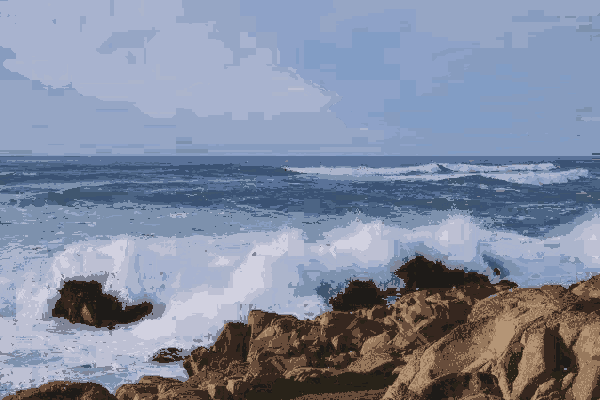
\includegraphics[width=90mm]{ocean-em-k20-60.png}
\end{figure}

\begin{figure}[ht!]
	\centering
	\caption{Ocean 50}
	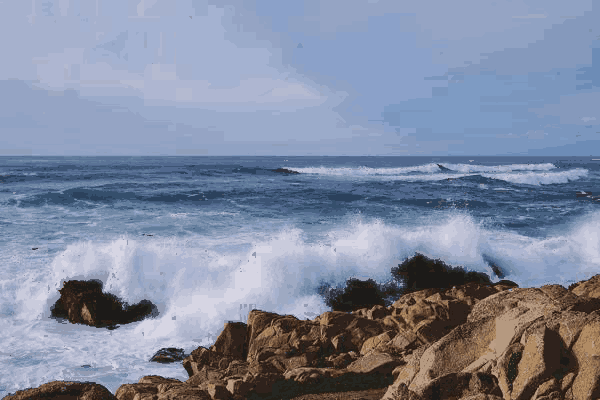
\includegraphics[width=90mm]{ocean-em-k50-24.png}
\end{figure}


\begin{figure}[ht!]
	\centering
	\caption{Polarlights 10}
	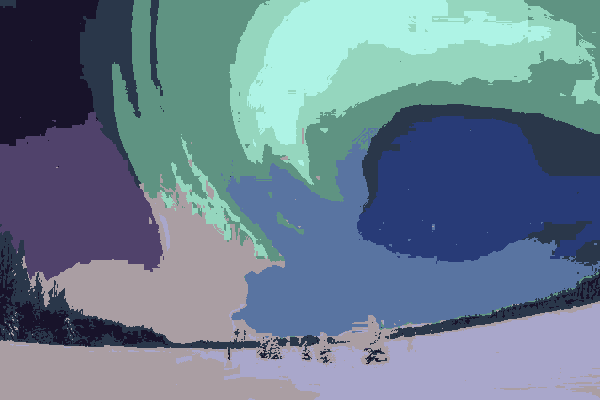
\includegraphics[width=90mm]{polarlights-em-k10-21.png}
\end{figure}

\begin{figure}[ht!]
	\centering
	\caption{Polarlights 20}
	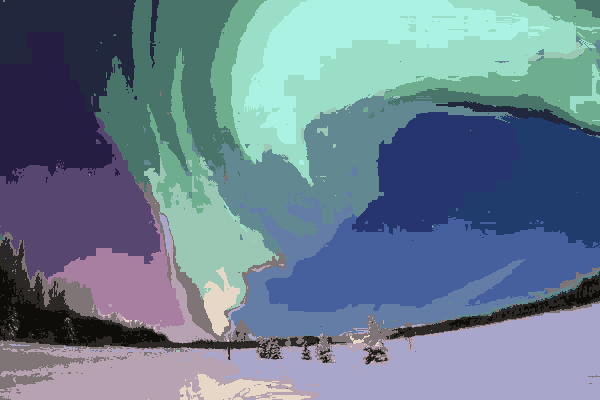
\includegraphics[width=90mm]{polarlights-em-k20-44.png}
\end{figure}

\begin{figure}[ht!]
	\centering
	\caption{Polarlights 50}
	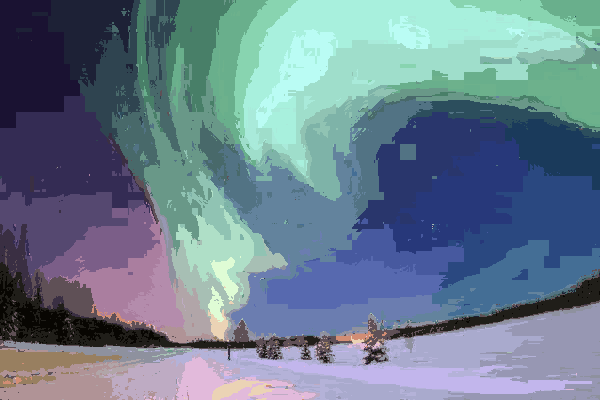
\includegraphics[width=90mm]{polarlights-em-k50-56.png}
\end{figure}

\begin{figure}[ht!]
	\centering
	\caption{Balloons 10}
	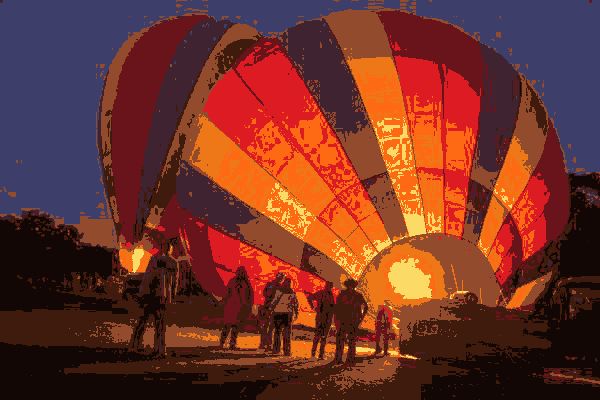
\includegraphics[width=90mm]{balloons-em-k10-26.png}
\end{figure}

\begin{figure}[ht!]
	\centering
	\caption{Balloons 20}
	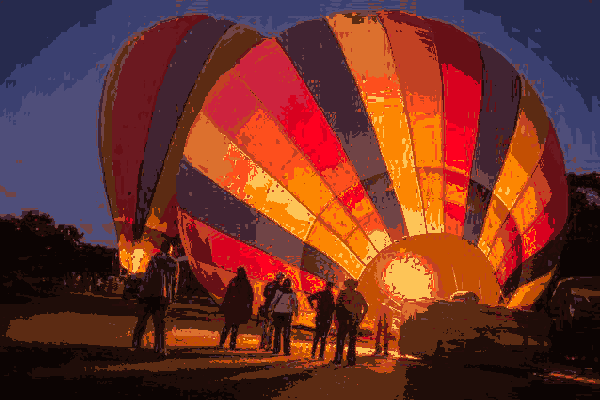
\includegraphics[width=90mm]{balloons-em-k20-100.png}
\end{figure}

\begin{figure}[ht!]
	\centering
	\caption{Balloons 50}
	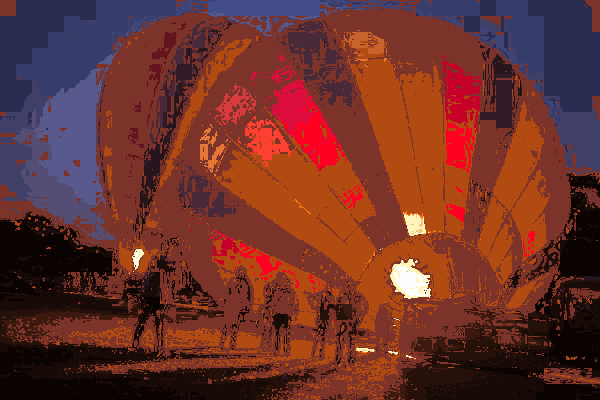
\includegraphics[width=90mm]{balloons-em-k50-100.png}
\end{figure}


\end{document}